\documentclass[dvisvgm,tikz]{standalone}
\usepackage{circuitikz}
\renewcommand{\familydefault}{\sfdefault}
\begin{document}
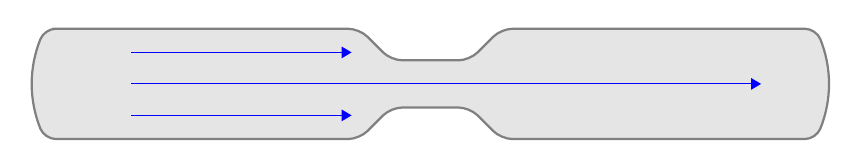
\begin{tikzpicture}
  % resistor
  \draw[rounded corners,thick,gray,fill=gray!20]
  ++(0,0)
  -- ++(3.9,0) -- ++(0.4,-0.4) -- ++(1,0) -- ++(0.4,0.4) -- ++(4,0)
  .. controls +(0.2,-0.5) and +(0.2,0.5) .. ++(0,-1.4)
  -- ++(-4,0) -- ++(-0.4,0.4) -- ++(-1,0) -- ++(-0.4,-0.4) -- ++(-4,0)
  .. controls +(-0.2,0.5) and +(-0.2,-0.5) .. ++(0,1.4)
  -- ++(0.1,0);
  \draw[blue, -Triangle] (1,-0.3) -- (3.8,-0.3);
  \draw[blue, -Triangle] (1,-0.7) -- (9,-0.7);
  \draw[blue, -Triangle] (1,-1.1) -- (3.8,-1.1);
\end{tikzpicture}
\end{document}